\documentclass[tikz,border=10pt]{standalone}
\usepackage[scaled=0.95]{helvet}
\renewcommand{\familydefault}{\sfdefault}
\usepackage[europeanresistors,americanvoltages]{circuitikz}
\definecolor{TEJNavy}{HTML}{1E2B55}
\definecolor{TEJBlue}{HTML}{1769AA}
\definecolor{TEJGold}{HTML}{D49B19}
\begin{document}
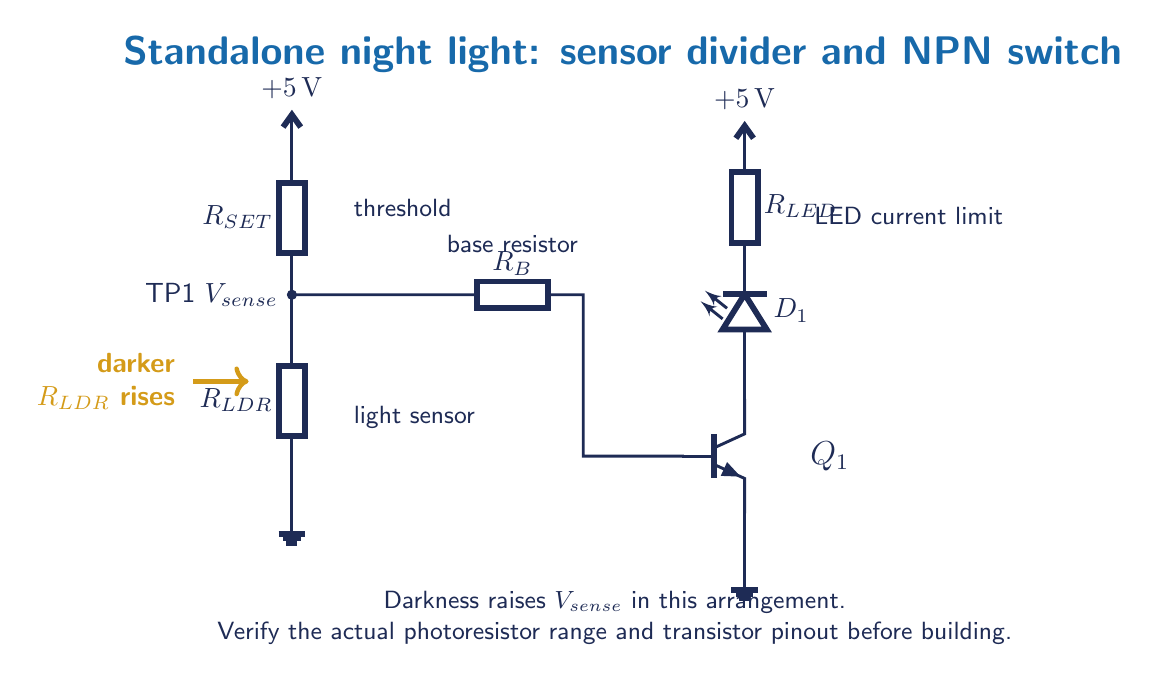
\begin{tikzpicture}[line width=1.05pt,draw=TEJNavy,text=TEJNavy,font=\sffamily]
  \ctikzset{bipoles/length=1.12cm}
  \node[font=\bfseries\Large,text=TEJBlue] at (5.7,7.3)
    {Standalone night light: sensor divider and NPN switch};

  % Sensor divider
  \draw (1.5,6.2) node[vcc] {$+5\,\mathrm{V}$}
    to[R,l_={$R_{SET}$}] (1.5,4.25)
    node[circ,label=left:{TP1 $V_{sense}$}] (sense) {}
    to[R,l_={$R_{LDR}$}] (1.5,1.55)
    node[ground] {};
  \node[anchor=west,font=\small] at (2.15,5.35) {threshold};
  \node[anchor=west,font=\small] at (2.15,2.7) {light sensor};

  % Transistor and load
  \node[npn,scale=1.15] (Q1) at (7.25,2.2) {};
  \node[anchor=west,font=\large] at (7.95,2.2) {$Q_1$};
  \draw (sense) -- (3.4,4.25)
    to[R,l={$R_B$}] (5.2,4.25)
    |- (Q1.B);
  \node[font=\small] at (4.3,4.9) {base resistor};
  \draw (Q1.E) -- ++(0,-0.65) node[ground] {};
  \draw (Q1.C) -- ++(0,0.5)
    to[leD,l_={$D_1$}] ++(0,1.25)
    to[R,l_={$R_{LED}$}] ++(0,1.4)
    node[vcc] {$+5\,\mathrm{V}$};
  \node[anchor=west,font=\small] at (8.0,5.25) {LED current limit};

  \draw[->,TEJGold,line width=1.6pt] (0.25,3.15) -- (0.95,3.15);
  \node[anchor=east,align=right,text=TEJGold,font=\bfseries] at (0.15,3.15)
    {darker\\$R_{LDR}$ rises};
  \node[align=center,font=\small] at (5.6,0.15)
    {Darkness raises $V_{sense}$ in this arrangement.\\
     Verify the actual photoresistor range and transistor pinout before building.};
\end{tikzpicture}
\end{document}
